\section{How to use EM Algorithm to solve Transcript Abundance Estimation}
The proof is credited to \cite{pachter2011models}.\\
Let $T$ be the set of transcripts from a RNA-sequencing samples and let $l_t$ be the length of transcript $t \in T$.\\
We define $\rho = \{\rho_t\}_{t \in T}$ be the relative abundances of transcripts such that $\sum_{t \in T}{\rho_t}=1$\\
Let $F$ be the set of reads and $F_t$ be the set of short reads from transcript $t \in T$ ($F_t \subseteq F$).\\
 Let there are $\lvert F \rvert$ reads of length $m$ on average. So, for a transcript $t \in T$, a read could start from $l_t-m+1$ possible locations. This will be denoted as the \textit{effective length} of transcript $t$, $\tilde{l_t}= l_t-m+1$.\\

\subsection{Expectation step} 
As per generative model assumptions, the probability of choosing a transcript $t$ for read is,
\begin{displaymath}
\frac{ {\rho_t}{\tilde{l_t}}  }{ \sum_{r \in T}{ {\rho_r}{\tilde{l_r}}} }
\end{displaymath}

There are $\tilde{l_t}$ possible places for a read from $t$ to start at. So the probability that a read was chosen from transcript $t$ is equal to the product of the probabilities of choosing $t$ and choosing a place from $t$ to start at,
\begin{displaymath}
\frac{ {\rho_t} {\tilde{l_t}}  }{ \sum_{r \in T} { {\rho_r}{\tilde{l_r}}} }
\times \frac{1}{\tilde{l_t}}
\end{displaymath}    

So, we will start the estimation process by assuming some initial values of hidden variables $\rho$.
\subsection{Maximization step}

So, for the set of reads from $t$, the number of reads is $X_t= \lvert F_t \rvert$.\\
To compute the likelihood of the parameter settings $\rho$, we need to compute the probabilities of $f \in F_t$ being generated from transcript $t$,
\begin{displaymath}
{({\frac{ {\rho_t} {\tilde{l_t}}  }{ \sum_{r \in T} { {\rho_r}{\tilde{l_r}}} }
\times \frac{1}{\tilde{l_t}}
})}^{X_t}
\end{displaymath}

So, the likelihood for parameter settings $\rho$ is,

\begin{displaymath} {\mathbf{L}(\rho)}=\prod_{t \in T}{{({\frac{ {\rho_t} {\tilde{l_t}}  }{ \sum_{r \in T} { {\rho_r}{\tilde{l_r}}} }
\times \frac{1}{\tilde{l_t}}
})}^{X_t}}
\end{displaymath}

Let, $\alpha_t=\frac{ {\rho_t} {\tilde{l_t}}  }{ \sum_{r \in T} { {\rho_r}{\tilde{l_r}}} }
$.\\So,
\begin{displaymath} {\mathbf{L}(\rho)}=\prod_{t \in T}{({\frac{\alpha_t}{\tilde{l_t}}) } ^{X_t} }
\end{displaymath} 
After applying log-likelihood and taking derivatives to find the maxima, we get,
\begin{displaymath}
\hat{\alpha_t}= \frac{{X_t}}{\sum_{t \in T}{{X_t}}}
\end{displaymath},

As ${\sum_{r \in T} { {\rho_r}{\tilde{l_r}}}}$ will be equal for each $t \in T$, we can write,
\begin{displaymath}
\hat{\alpha_t} \propto {{\hat{{\rho_t}} { \tilde{l_t} } } }
\implies  \hat{\rho_t} \propto {{\frac{\hat{\alpha_t}}{\tilde{l_t}}}}
\end{displaymath}
From this calculation, we can re-estimate the value of $\rho$ and use it in next iteration of EM until convergence.

\begin{figure}[h]
\centering
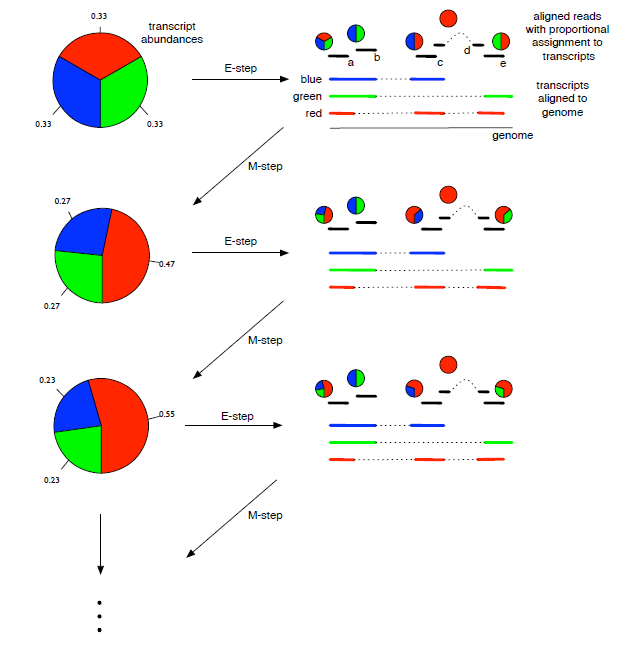
\includegraphics[scale=0.60]{ex.png}
\caption{EM in Transcription Abundance Estimation~\cite{pachter2011models}}
\label{}
\end{figure}